\chapter{Implementation}
\label{chapter:implementation}



TODO Some text here for latex placement

% ###############################################################
\section{Upgrading Kubric to use Blender to version 3.1}
\label{sec:upgrading-kubric}

% ###############################################################
\section{Downloading Geographic Data}
\label{sec:dowonload-geo-data}

TODO Some text here for latex placement

% ###############################################################
\section{Saving and Restoring Blender Geometry Nodes}
\label{sec:save-restore-blender-geometry}

TODO Some text here for latex placement


% ###############################################################
\section{Combining Levels of Detail}
\label{sec:combine-levels-of-detail}

TODO Some text here for latex placement

\begin{figure}[H]
    \centering
    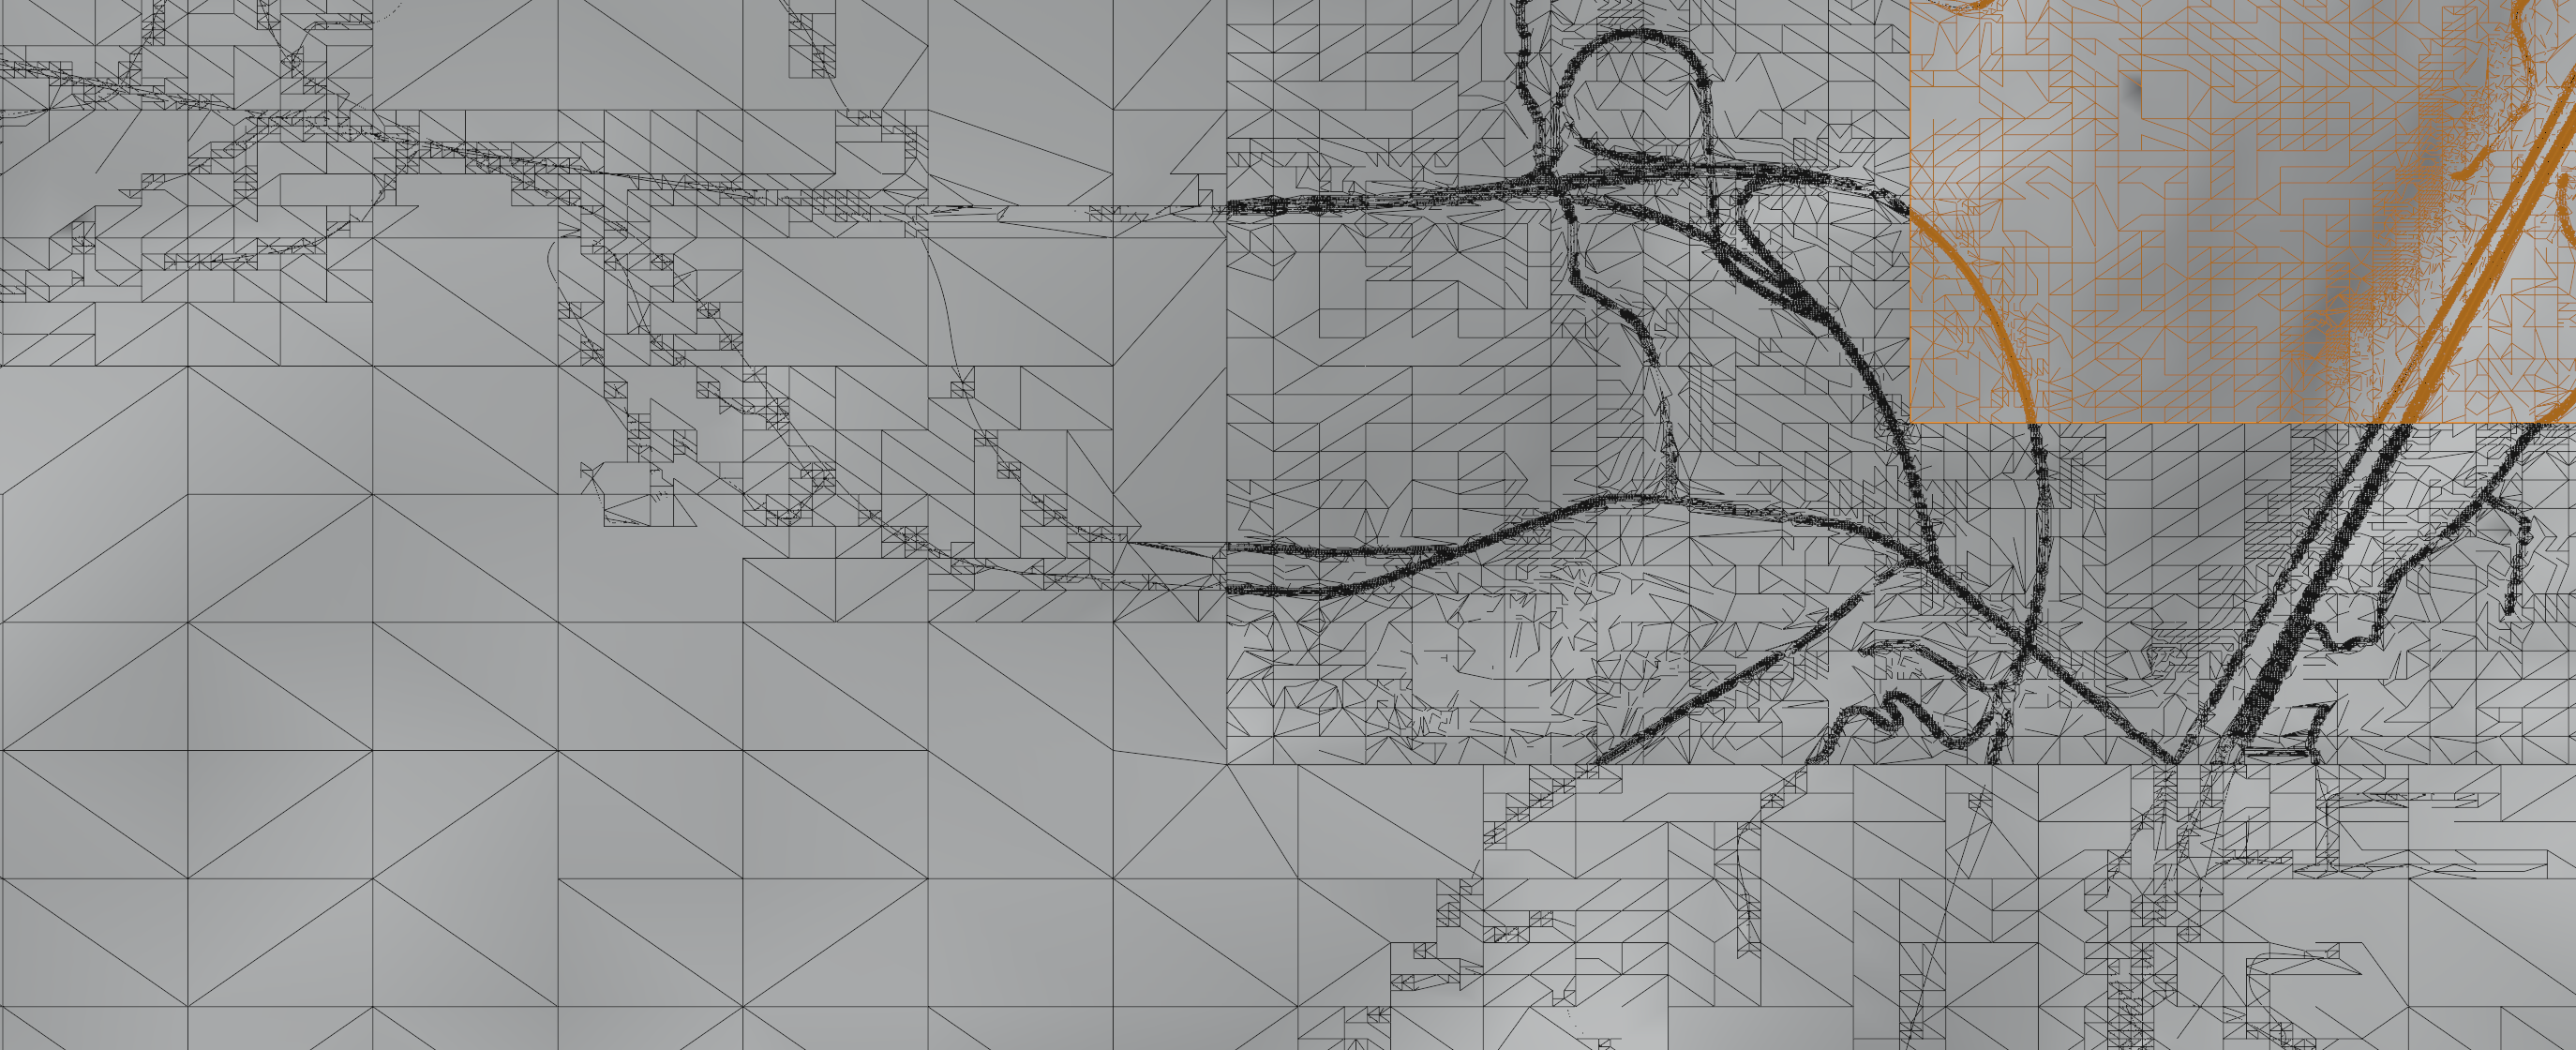
\includegraphics[width=14.5cm]{src/img/pic/pic-1 blender screenshot sat levels of detail.png}
    \caption{Different levels of detail }
    \label{fig:impl-levels-of-detail}
\end{figure}

TODO Some text here for latex placement

\begin{figure}[H]
    \centering
    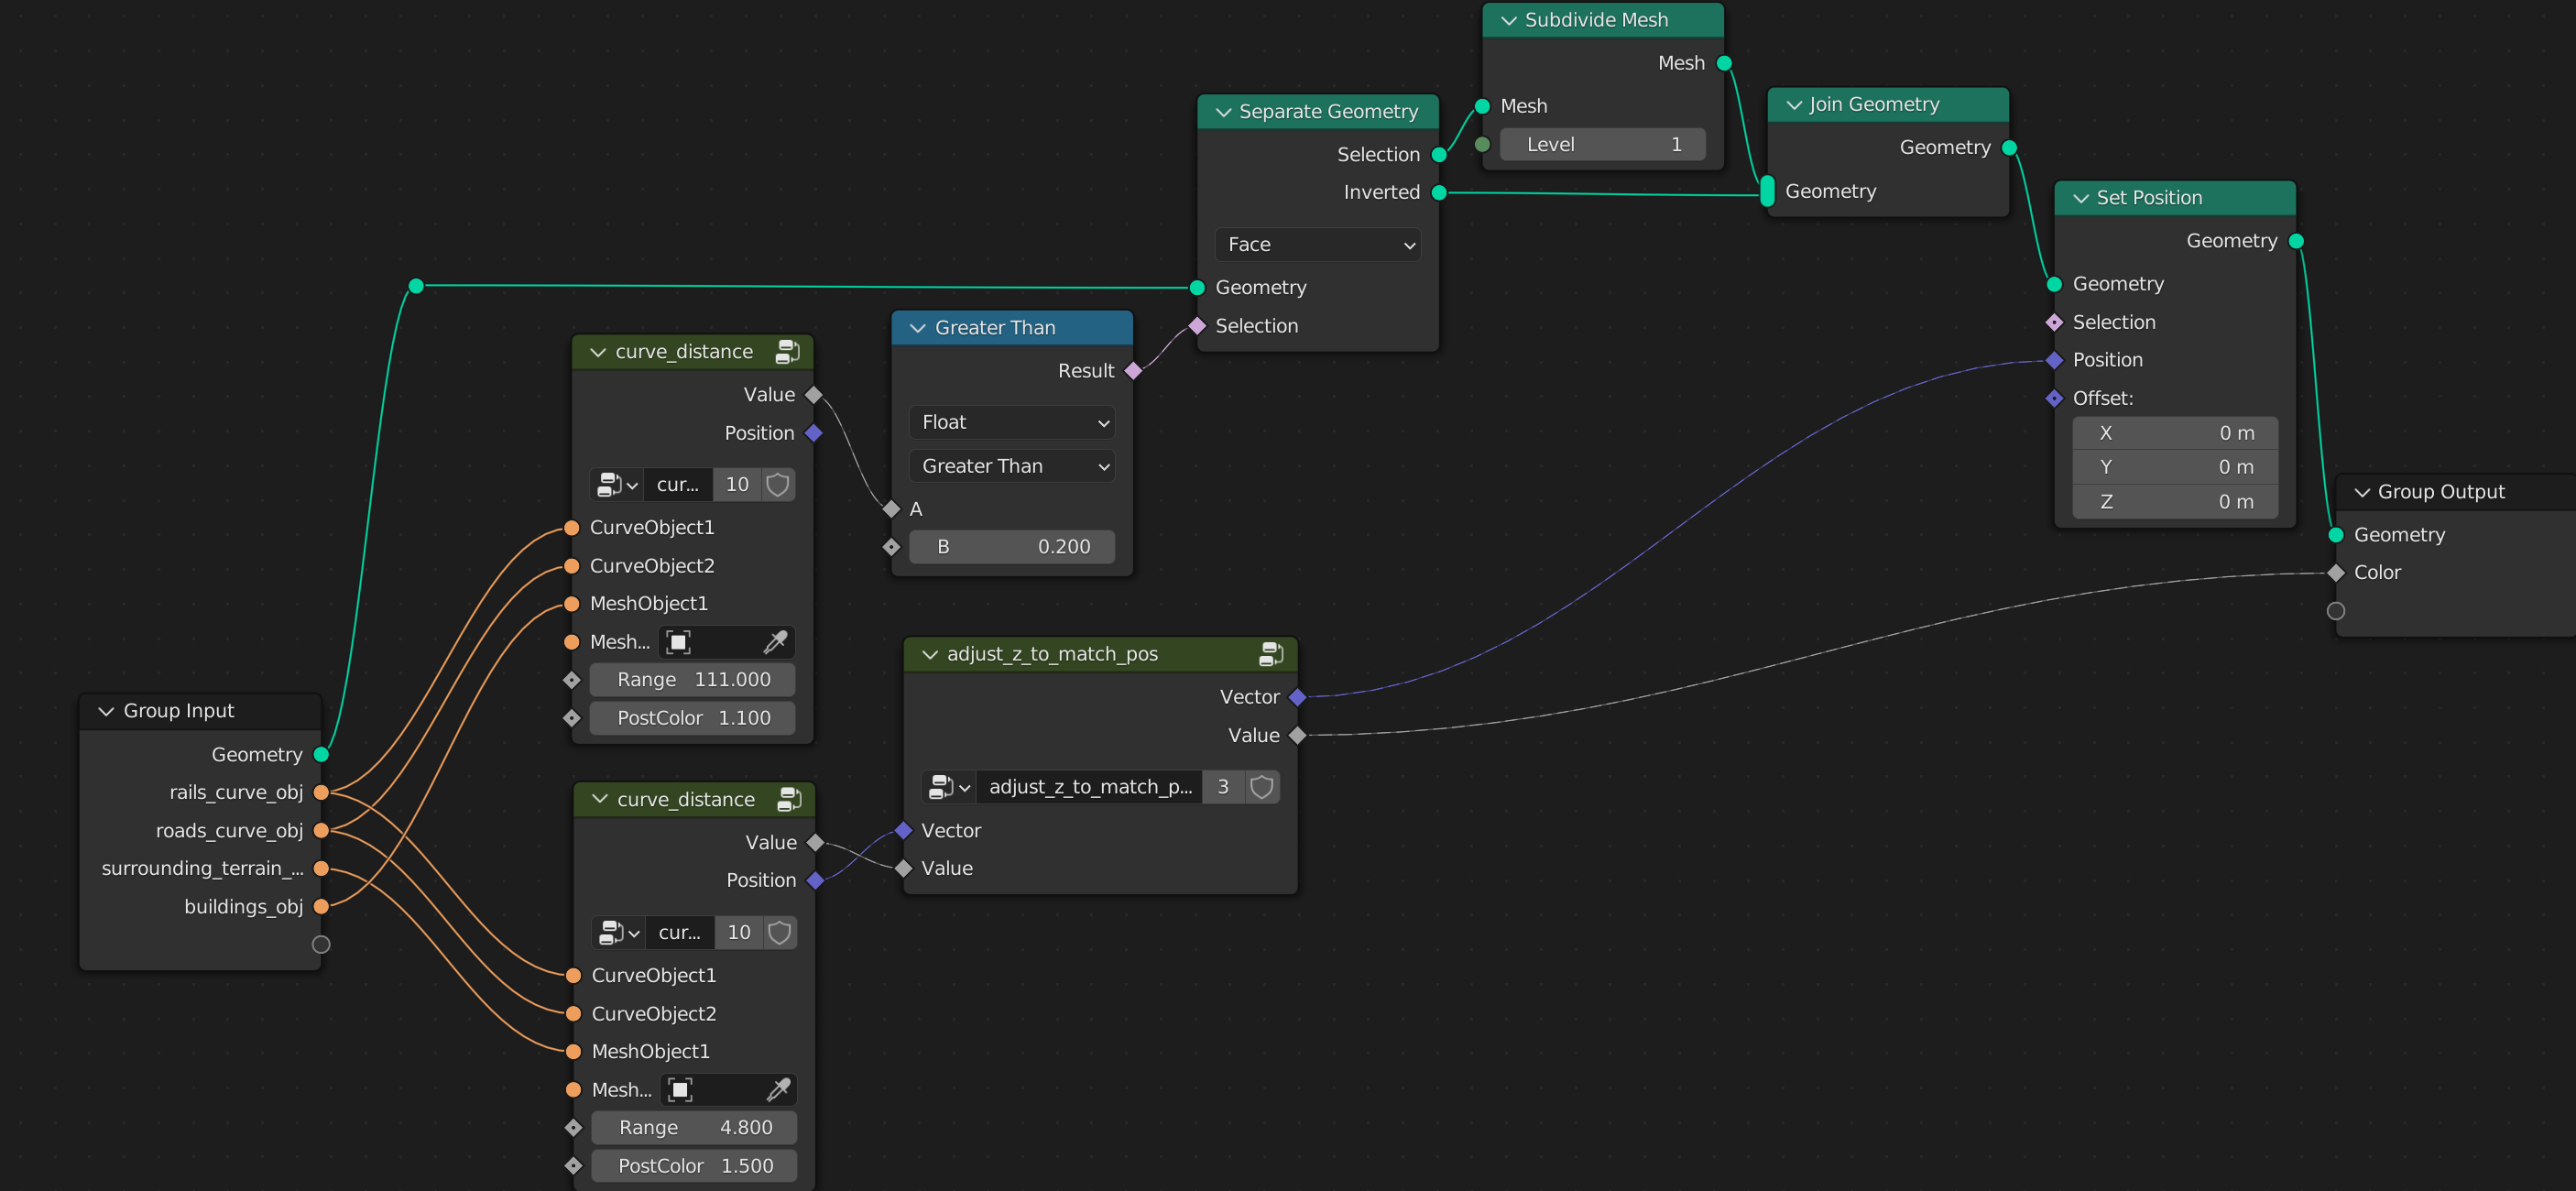
\includegraphics[width=14.5cm]{src/img/pic/pic-2 screenshot of blender adjust terrain geometry node.png}
    \caption{Geometry Node Implementation for terrain height adjustment and tessellation}
    \label{fig:impl-geom-nodes-terrain}
\end{figure}


TODO Some text here for latex placement


\begin{figure}[H]
    \centering
    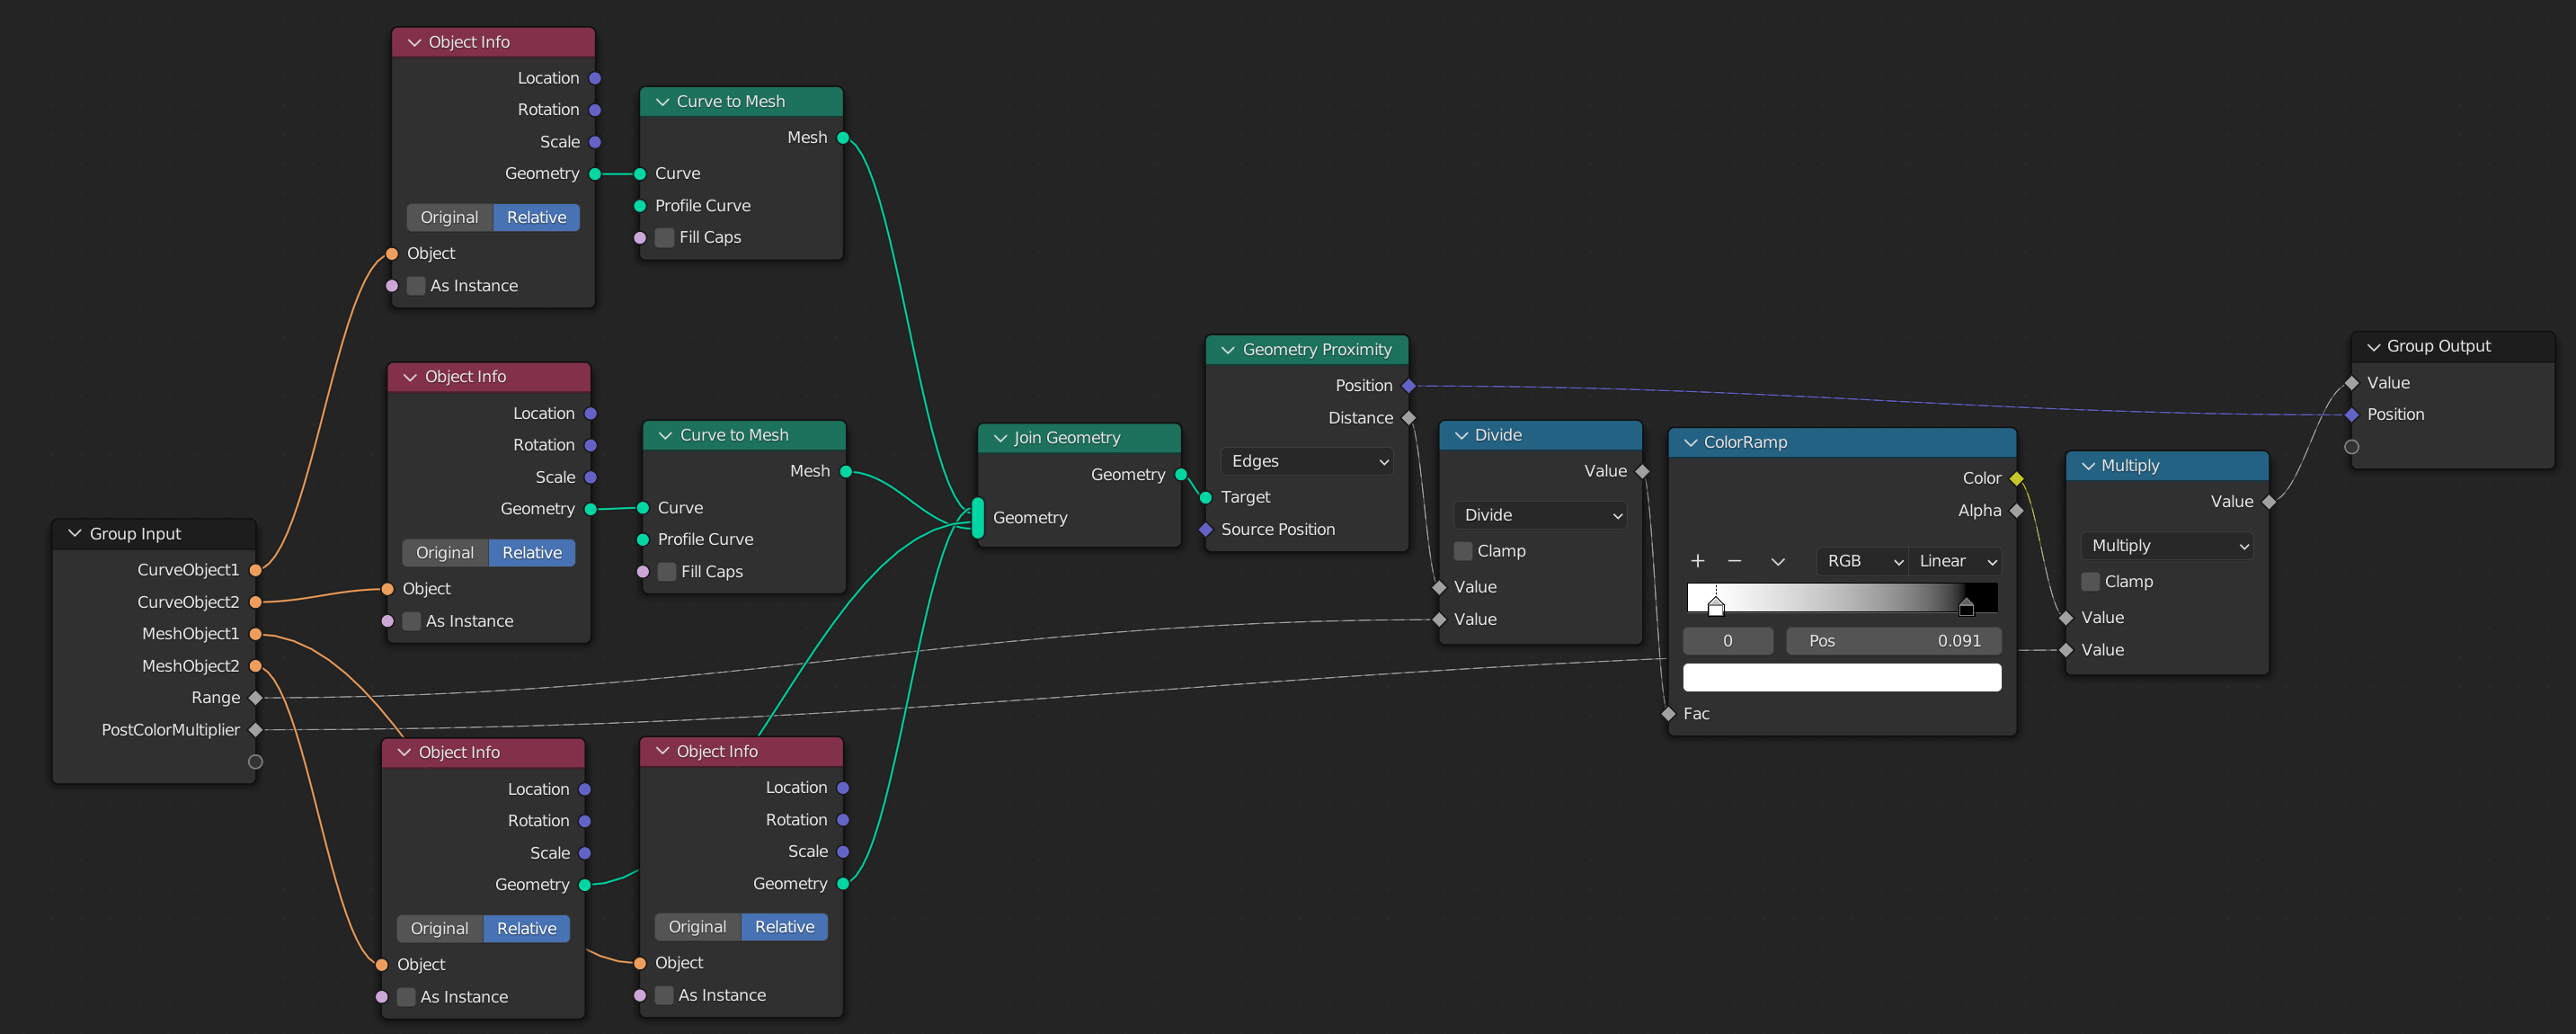
\includegraphics[width=14.5cm]{src/img/pic/pic-3 blender geometry screenshot curve_distance.png}
    \caption{Geometry Node Implementation for curve_distance}
    \label{fig:impl-curve-dist}
\end{figure}

\begin{figure}[H]
    \centering
    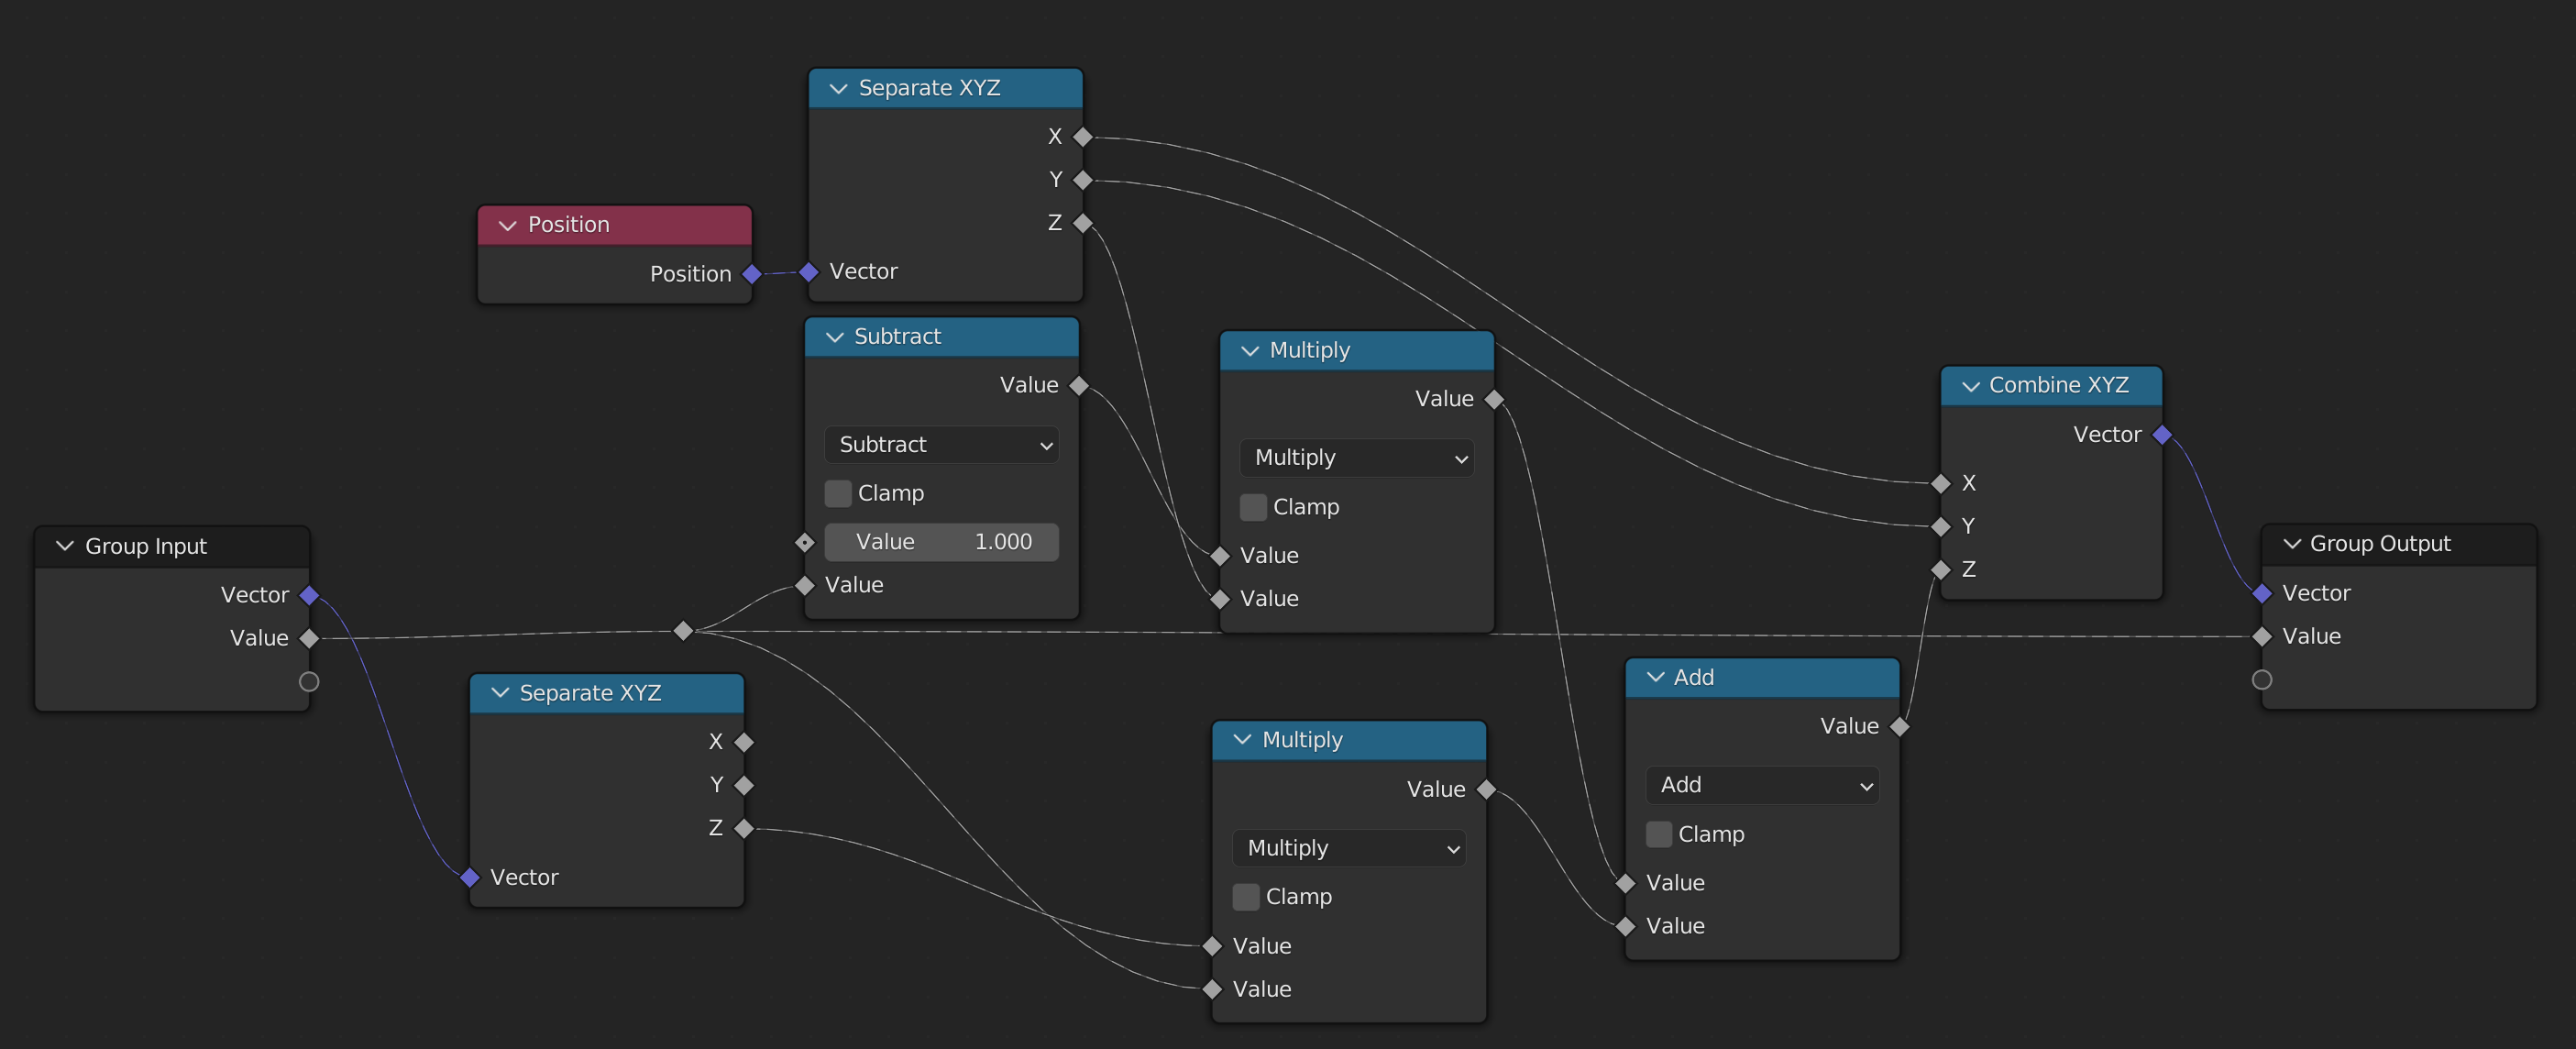
\includegraphics[width=14.5cm]{src/img/pic/pic-4 blender geometry node screenshot adjust_z_to_match_pos.png}
    \caption{Geometry Node Implementation for adjust_z_to_match_pos}
    \label{fig:impl-adjust-z-to-match-pos}
\end{figure}


TODO Some text here for latex placement


% ###############################################################
\section{Procedural Railway Generation}
\label{sec:procedural-railway-generation}

TODO planks

TODO rails

TODO signage



% ###############################################################
\section{Vegetation Scatter and Geometry Caching}
\label{sec:vegetation-scatter}


TODO veg


% ###############################################################
\section{Scene Setup and Rendering Loop}
\label{sec:rendering}


TODO render loop / interactive
